\section{Context Oriented nesC (ConesC)} To mention: detailed description of
ConesC, using Wildlife tracking application.

Programming in ConesC is tightly coupled with environment-dependent behavior of
the application and exploits two main concepts: \emph{i)} individual contexts
and their transitions and \emph{ii)} context groups. The former represent
different environment situations where a system may find itself. Each context
maps a separate state of application-level or system-level. As the environment
conditions change, a programmer initiates a context transition by
\emph{activating} corresponding context. Context group is a set of contexts
sharing common characteristics. Thus, whenever a transition between involved
contexts occurs it is determined by changes in the same physical quantity.

Diagram on a figure~\ref{fig:wtd} displays contextual situations, which may
occur during the execution. To reflect this diagram on a language level, ConesC
utilizes new types of components, such as \emph{context} and \emph{context
configuration}, and a set of new key-words. \emph{Context} and \emph{context
group} types are extensions of \emph{module} and \emph{configuration}
correspondingly. Their instances however can also be used as standard nesC
components. E.g. they can provide or use interfaces as well as be declared in
the same way.

\begin{figure}[!h]
\centering
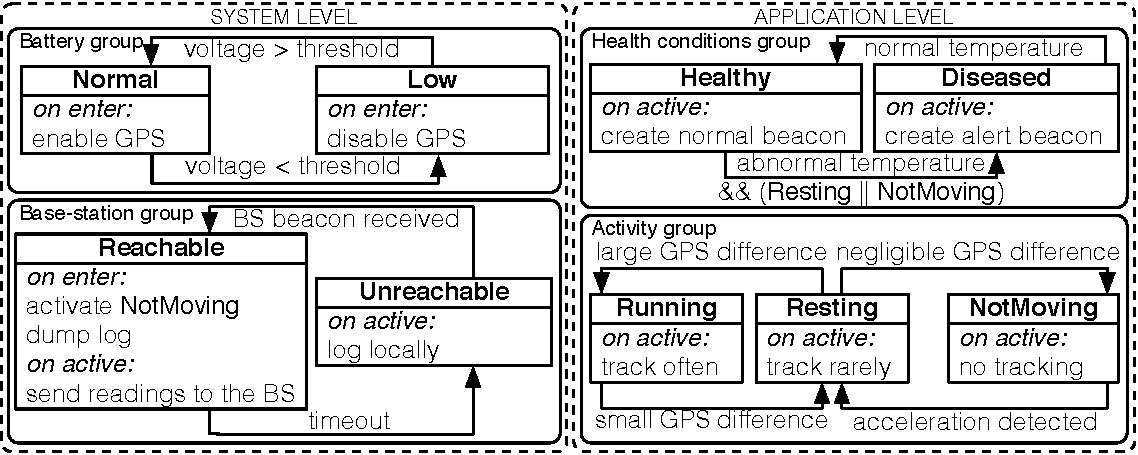
\includegraphics[width=\columnwidth]{pdf/wildlifetracking}
\caption{Wildlife tracking diagram.}
\label{fig:wtd}
\end{figure}

\subsection{Context and Context configuration}

\emph{Context configuration} component (figure~\ref{fig:ccc}) logically
represents a context group and is intended to declare layered functions as well
as included contexts. Here key-word \emph{layered} (line~\lstref{layereddef})
means that the behavior of this function depends on activated context. The
declaration of contexts (line~\lstref{contexts}) follows a key-word
\emph{contexts}, but it can also be moved in \emph{components} declaration,
since the key-word \emph{contexts} was introduced only for convenience and
\emph{context} can be declared as a standard component. It is mandatory,
however, to declare \emph{default} context (line~\lstref{isdefault}), which will
be activated at the beginning of the execution, by using key-word \emph{is
default}. ConesC also supports a declaration of \emph{error}
(line~\lstref{iserror}) context for each group by the key-word \emph{is error}.
Error context is used to indicate errors occurred during the execution. If error
context is not declared, it will be generated automatically.

\begin{figure}[!tb]
\begin{lstlisting}[style=conescframe]
context group BaseStationG {
*\lstnote{layereddef}*  layered command void report(msg_t msg);
}implementation {
*\lstnote{contexts}*  contexts InRange,
*\lstnote{isdefault}*    OutRange is default,
*\lstnote{iserror}*    ErrorC is error;
 components Routing, Logging, LedsC;
 InRange.Collection -> Routing;
 OutRange.DataStore -> Logging;
 Error.Leds -> LedsC;}
\end{lstlisting}
\vspace{-4mm}
\caption{Context configuration component.}
  \label{fig:ccc}
\vspace{-2mm}
\end{figure}
\begin{figure}[!h]
\TheSbox
\caption{Context configuration
component.}
\label{fig:ccc}
\end{figure}

\emph{Context} component (figure~\ref{fig:cc}) includes a context-specific
implementation of layered function (line~\lstref{layeredimp}) declared in
context configuration. Since only one context in a group can be active at a
time, a behavioral variation is enabled by this implementation. In our example,
function \emph{report()} deposits a message in local memory while \emph{No Base
Station} context is active. Programmer may want to add some instructions after
context activation such as initialization of variables or enabling/disabling
modules (in our example, enable GPS-sensor on entering in \emph{no BS} context).
Or it may be necessary to reset component's state before context deactivation.
ConesC allows to do this by implementing events \emph{activated()} and
\emph{deactivated()} correspondingly (lines~\lstref{activated}
and~\lstref{deactivated}), it is not obligatory though.

In order to double check if context is really taking place during a context
transition and avoid false positives, ConesC provides a \emph{check()} command
(line~\lstref{check}). It is also not mandatory to implement this command, but
should it return \emph{FALSE}, an initiated context transition will not occur, a
context will not be activated and a system will remain in the previous state.
This approach allows one not to think about conditions a transition taking place
in, but foresee possible conflicts.

\begin{figure}[!tb]
\begin{lstlisting}[style=conescframe]
context OutRange {
*\lstnote{dependence}*  transitions InRange iff ActivityG.Running;
  uses interface DataStore;
}implementation {
*\lstnote{activated}*  event void activate(){
  //...}
*\lstnote{deactivated}*  event void deactivate(){
  //...}
*\lstnote{layeredimp}*  layered command void report(msg_t msg){
    call DataStore.deposit(msg);}}
\end{lstlisting}
\vspace{-4mm}
\caption{Context component.}
  \label{fig:cc}
\vspace{-2mm}
\end{figure}
\begin{figure}[!h]
\TheSbox
\caption{Context component.}
\label{fig:cc}
\end{figure}

\subsection{Transition rules}

Along with declaration of a new component types, ConesC also allows to specify
rules and dependencies for context transitions. In our application for example
within \emph{Activity} group a transition from \emph{not moving} to
\emph{resting} is only possible. Since each transition is governed by a separate
rule, it is declared in context component as shown on figure~\ref{fig:nmc}
(line~\lstref{transitions}). Here key-word \emph{transitions} indicates a list
of possible contexts a transition can be performed to. If programmer initiates a
transition to a context which is not declared in the rule, an \emph{error}
context will be activated.

\begin{figure}[!tb]
\begin{lstlisting}[style=conescframe]
context NotMoving {
*\lstnote{transitions}*  transitions Resting;
}implementation {
 //..}
\end{lstlisting}
\vspace{-4mm}
\caption{NotMoving context.}
  \label{fig:nmc}
\vspace{-2mm}
\end{figure}
\begin{figure}[!h]
\TheSbox
\caption{NotMoving context.}
\label{fig:nmc}
\end{figure}

To map intergroup relations we are introducing a context transition dependencies
in our context-oriented language. Within the \emph{Base Station} group for
example a transition from \emph{no Base Station} to \emph{Base Station} is only
possible if an animal is \emph{running}. Thus, the dependency for this
transition is \emph{running} context, which belongs to \emph{Activity} group.
Our approach also covers this type of situations by adding dependencies to the
transition declaration as it is shown on a figure~\ref{fig:cc}
(line~\lstref{dependence}). In \emph{transitions} section a context name
followed by a key-word \emph{iff} and full name of another context means that
the transition will only be executed if the latter context is active. Should the
rule with dependency be violated, a transition to an error context will be
triggered.

Other type of intergroup relations implies automatic triggering of context
transition. Considering \emph{battery} group in our example, we can notice that
for further energy saving programmer may want to trigger a transition to
\emph{No Base Station} context withing a \emph{Base Station} group as long as
\emph{Low} context is active. Our design allows one to do that by declaring a
\emph{triggers} section. On a figure~\ref{fig:cc} (line~\lstref{triggers}) all
the declared after this key-word contexts will be activated as soon as a
transition to the current context is triggered, all declared rules are
satisfied, and implemented \emph{check()} command returns \emph{TRUE}.

\begin{Sbox}
\begin{minipage}{\columnwidth}
\begin{csource}
(*@\textbf{context}@*) Low {
 (*@\lstnote{triggers}\textbf{triggers}@*) BaseStationG.OutRange;
}implementation {
 //..}
\end{csource}
\end{minipage}
\end{Sbox}
\begin{figure}[!h]
\TheSbox
\caption{Low context.}
\label{fig:lc}
\end{figure}

\subsection{Usage}

This section shows how ConesC structures can be used to invoke a behavioral
variation. Here we describe one aspect of an application's behavioral variation
which is related to the Base Station availability. As it was mentioned before,
if a node receives a beacon from the Base Station it activates \emph{Base
Station} context, and \emph{no Base Station} context in case of timeout.
Programmer however can not operate by contexts directly, but should use
\emph{context group}, which is \emph{BaseStationG} in our example. In the main
configuration (figure~\ref{fig:mc}) base station group is declared
(line~\lstref{declaration}) and wired (line~\lstref{wiring}) as a standard
component, since it is an extension of a configuration.

\begin{Sbox}
\begin{minipage}{\columnwidth}
\begin{csource}
(*@\textbf{configuration}@*) ApplicationC {
}implementation {
  (*@\lstnote{declaration}\textbf{components}@*) BaseStationG, Application;
  //...
  (*@\lstnote{wiring}@*)Application.BaseStationG -> BaseStationG;
}
\end{csource}
\end{minipage}
\end{Sbox}
\begin{figure}[!h]
\TheSbox
\caption{Main configuration.}
\label{fig:mc}
\end{figure}

In the main module (figure~\ref{fig:mm}) however it is necessary to declare
explicitly that we are using a context group \emph{BaseStationG}
(line~\lstref{cgdecl}). Activation of a context initiates by using a key-word
\emph{activate} which is followed by a full context name. Thus
\emph{BaseStation} context is activated on the line~\lstref{actBS} as soon as a
beacon from the base station received. But should timeout occur, context
\emph{NoBaseStation} will be activated (line~\lstref{actNoBS}). The benefit of
this approach is that layered function can be called independently
(line~\lstref{calling}), and activating code is kept separately from function
calls. Moreover one should not care about the base station availability, while
reporting measured data, since the behavior of layered function
\emph{BaseStationG.report()} depends on activated context, e.g. the base station
availability.

It is also obligated to implement event \emph{contextChanged()} for each used
context group, as we did on the line~\lstref{eventCC}. This event is fired every
time when context changes. Context in this scope is considered as a constant,
whose name consists of two parts, joined by a dot: a name of a group and a name
of a context. Thus, in function \emph{BaseStationG.contextChanged()} we can use
a passed parameter \emph{con} to find out what context has been activated, as
shown on line~\lstref{concheck}.

\begin{Sbox}
\begin{minipage}{\columnwidth}
\begin{csource}
(*@\textbf{module}@*) Application {
  (*@\lstnote{cgdecl}@*)uses (*@\textbf{context group}@*) BaseStationG;
   //...
}implementation {
   //...
   event void Timer.fired() {
  (*@\lstnote{calling}@*) call BaseStationG.report(msg);}
  (*@\lstnote{eventCC}@*)event void BaseStationG.contextChanged(context_t con) {
  (*@\lstnote{concheck}@*) if(con == BaseStationG.InRange)
      dbg("Debug", "Base station is within the range!");}}
\end{csource}
\end{minipage}
\end{Sbox}
\begin{figure}[!h]
\TheSbox
\caption{Main module.}
\label{fig:mm}
\end{figure}
